\documentclass[11pt,twoside]{report}

% some definitions for the title page
\newcommand{\reporttitle}{Transfer Learning for bespoke automatic contouring of cervical cancer radiotherapy planning}
\newcommand{\reportauthor}{Anton Zhitomirsky}
\newcommand{\supervisor}{Ben Glocker}
\newcommand{\secondMarker}{TODO}
\newcommand{\reporttype}{MEng Individual Project}

\usepackage{pifont,mdframed}
\newenvironment{warning}
  {\par\begin{mdframed}[linewidth=1pt,linecolor=black]%
    \begin{list}{}{\leftmargin=1cm
                   \labelwidth=\leftmargin}\item[\Large\ding{43}]}
  {\end{list}\end{mdframed}\par}

% load some definitions and default packages
%%%%%%%%%%%%%%%%%%%%%%%%%%%%%%%%%%%%%%%%%
% University Assignment Title Page 
% LaTeX Template
% Version 1.0 (27/12/12)
%
% This template has been downloaded from:
% http://www.LaTeXTemplates.com
%
% Original author:
% WikiBooks (http://en.wikibooks.org/wiki/LaTeX/Title_Creation)
%
% License:
% CC BY-NC-SA 3.0 (http://creativecommons.org/licenses/by-nc-sa/3.0/)
% 
%
%%%%%%%%%%%%%%%%%%%%%%%%%%%%%%%%%%%%%%%%%
%----------------------------------------------------------------------------------------
%	PACKAGES AND OTHER DOCUMENT CONFIGURATIONS
%----------------------------------------------------------------------------------------
\usepackage[a4paper,hmargin=2.0cm,vmargin=1.0cm,includeheadfoot]{geometry}
\usepackage{textpos}

\usepackage[square,numbers]{natbib} % for bibliography
\usepackage[nottoc]{tocbibind} % Includes "References" in the table of contents
\bibliographystyle{unsrtnat}

\usepackage{tabularx,longtable,multirow,subfigure,caption}%hangcaption
\usepackage{fancyhdr} % page layout
\usepackage{url} % URLs
\usepackage[english]{babel}
\usepackage{amsmath}
\usepackage{graphicx}
\usepackage{scalerel}
\usepackage{dsfont}
\usepackage{epstopdf} % automatically replace .eps with .pdf in graphics
\usepackage{backref} % needed for citations
\usepackage{array}
\usepackage{latexsym}

\usepackage[pdftex,pagebackref,hypertexnames=false,colorlinks]{hyperref} % provide links in pdf
\usepackage{booktabs}
\usepackage{wrapfig}
\usepackage{caption}  % Required for \captionof
\usepackage{float} % for H option in figures
\usepackage{amssymb}
\usepackage{amsmath}
\usepackage{csquotes}
% \usepackage{subcaption} % causes a compilation error after changing back to natbib referencing... 

\hypersetup{pdftitle={},
  pdfsubject={}, 
  pdfauthor={},
  pdfkeywords={}, 
  pdfstartview=FitH,
  pdfpagemode={UseOutlines},% None, FullScreen, UseOutlines
  bookmarksnumbered=true, bookmarksopen=true, colorlinks,
    citecolor=black,%
    filecolor=black,%
    linkcolor=black,%
    urlcolor=black}

\usepackage[all]{hypcap}

%%%%%%%%%%%%%%%%%%%%%%%%%%%%%%%%%%%%%%%%%%%%%%%%%%%%%%%%%%%%%%%%%%%%%%%%%%%%%%%%
% LISTINGS ammendments
%%%%%%%%%%%%%%%%%%%%%%%%%%%%%%%%%%%%%%%%%%%%%%%%%%%%%%%%%%%%%%%%%%%%%%%%%%%%%%%%
\usepackage{listings}

\lstset
{ %Formatting for code in appendix
    language=Matlab,
    basicstyle=\footnotesize,
    % numbers=left,
    stepnumber=1,
    showstringspaces=false,
    tabsize=1,
    breaklines=true,
    breakatwhitespace=false,
    frame=single,
    columns=fullflexible,
    postbreak=\mbox{\textcolor{red}{$\hookrightarrow$}\space},
}

%\usepackage{color}
%\usepackage[tight,ugly]{units}
%\usepackage{float}
%\usepackage{tcolorbox}
%\usepackage[colorinlistoftodos]{todonotes}
% \usepackage{ntheorem}
% \theoremstyle{break}
% \newtheorem{lemma}{Lemma}
% \newtheorem{theorem}{Theorem}
% \newtheorem{remark}{Remark}
% \newtheorem{definition}{Definition}
% \newtheorem{proof}{Proof}


%%% Default fonts
\renewcommand*{\rmdefault}{bch}
\renewcommand*{\ttdefault}{cmtt}


%%% Default settings (page layout)
\setlength{\parindent}{0em}  % indentation of paragraph
\setlength{\parskip}{.3em}

% \setlength{\parindent}{0em}  % indentation of paragraph

\setlength{\headheight}{14.5pt}
\pagestyle{fancy}
\renewcommand{\chaptermark}[1]{\markboth{\chaptername\ \thechapter.\ #1}{}}
%\fancyhead[RO]{\sffamily \textbf{\thepage}} %Page no.in the right on even pages
%\fancyhead[LE]{\sffamily \textbf{\thepage}} %Page no. in the left on odd pages

\fancyfoot[ER,OL]{\thepage}%Page no. in the left on
%odd pages and on right on even pages
\fancyfoot[OC,EC]{\sffamily }
\renewcommand{\headrulewidth}{0.1pt}
\renewcommand{\footrulewidth}{0.1pt}
\captionsetup{margin=10pt,font=small,labelfont=bf}


%--- chapter heading

\def\@makechapterhead#1{%
  \vspace*{10\p@}%
  {\parindent \z@ \raggedright \sffamily
    \interlinepenalty\@M
    \Huge\bfseries \thechapter \space\space #1\par\nobreak
    \vskip 30\p@
  }}

%--- chapter heading

\def\@makechapterhead#1{%
  \vspace*{10\p@}%
  {\parindent \z@ \raggedright \sffamily
    %{\Large \MakeUppercase{\@chapapp} \space \thechapter}
    %\\
    %\hrulefill
    %\par\nobreak
    %\vskip 10\p@
    \interlinepenalty\@M
    \Huge\bfseries \thechapter \space\space #1\par\nobreak
    \vskip 30\p@
  }}

%---chapter heading for \chapter*  
\def\@makeschapterhead#1{%
  \vspace*{10\p@}%
  {\parindent \z@ \raggedright
    \sffamily
    \interlinepenalty\@M
    \Huge \bfseries  #1\par\nobreak
    \vskip 30\p@
  }}
\allowdisplaybreaks

% load some macros
% Here, you can define your own macros. Some examples are given below.

\newcommand{\R}[0]{\mathds{R}} % real numbers
\newcommand{\Z}[0]{\mathds{Z}} % integers
\newcommand{\N}[0]{\mathds{N}} % natural numbers
\newcommand{\C}[0]{\mathds{C}} % complex numbers
% \renewcommand{\vec}[1]{{\boldsymbol{{#1}}}} % vector
\newcommand{\mat}[1]{{\boldsymbol{{#1}}}} % matrix

\usepackage{pifont,mdframed}
\newenvironment{warning}
  {\par\begin{mdframed}[linewidth=1pt,linecolor=black]%
    \begin{list}{}{\leftmargin=1cm
                  \labelwidth=\leftmargin}\item[\Large\ding{43}]}
  {\end{list}\end{mdframed}\par}

\definecolor{lightgray}{gray}{0.9}

\addbibresource{../../research/source/bibliography.bib}

% load title page
\begin{document}
% Last modification: 2015-08-17 (Marc Deisenroth)
\begin{titlepage}

    \newcommand{\HRule}{\rule{\linewidth}{0.5mm}} % Defines a new command for the horizontal lines, change thickness here
    
    %----------------------------------------------------------------------------------------
    %	LOGO SECTION
    %----------------------------------------------------------------------------------------
    
    
\includegraphics[width = 4cm]{../figures/imperial.pdf}\\[0.5cm] 
    
    \center % Center everything on the page
     
    %----------------------------------------------------------------------------------------
    %	HEADING SECTIONS
    %----------------------------------------------------------------------------------------
    
    \textsc{\LARGE \reporttype}\\[1.5cm] 
    \textsc{\Large Department of Computing}\\[0.5cm] 
    \textsc{\large Imperial College of Science, Technology and Medicine}\\[0.5cm] 
    
    %----------------------------------------------------------------------------------------
    %	TITLE SECTION
    %----------------------------------------------------------------------------------------
    
    \HRule \\[0.4cm]
    { \huge \bfseries \reporttitle}\\ % Title of your document
    \HRule \\[1.5cm]
     
    %----------------------------------------------------------------------------------------
    %	AUTHOR SECTION
    %----------------------------------------------------------------------------------------
    
    \begin{minipage}{0.4\textwidth}
    \begin{flushleft} \large
    \emph{Author:}\\
    \reportauthor % Your name
    \end{flushleft}
    \end{minipage}
    ~
    \begin{minipage}{0.4\textwidth}
    \begin{flushright} \large
    \emph{Supervisor:} \\
    \supervisor % Supervisor's Name
    \end{flushright}
    \end{minipage}\\[4cm]
    
    
    
    
    %----------------------------------------------------------------------------------------
    
    
    %----------------------------------------------------------------------------------------
    %	DATE SECTION
    %----------------------------------------------------------------------------------------
    
    {\large \today} % Date, change the \today to a set date if you want to be precise
    
    
    \vfill % Fill the rest of the page with whitespace
    Submitted in partial fulfillment of the requirements for the \degreetype~of Imperial College London
    
    \end{titlepage}
    


% page numbering etc.
\pagenumbering{roman}
\clearpage{\pagestyle{empty}\cleardoublepage}
\setcounter{page}{1}
\pagestyle{fancy}

% \cleardoublepage
%%%%%%%%%%%%%%%%%%%%%%%%%%%%%%%%%%%%
% \section*{Acknowledgments}
% Comment this out if not needed.

% \clearpage{\pagestyle{empty}\cleardoublepage}

%%%%%%%%%%%%%%%%%%%%%%%%%%%%%%%%%%%%
\begin{abstract} \label{sect:abstract}
  Clinicians target cancerous tumours by studying 3D contrasting images of cancerous tumours and surrounding soft tissues to plan targets for radiation therapy. The Royal Marsden Hospital is a key contributor of data for this project, which uses this approach to delineate tumours for cervical cancers. Typically after a gross tumour volume (GTV) is extrapolated from the relevant imaging modality, clinicians append tailored safety margins to also account for the microscopic cancerous spreads not visible in the scan to generate the planned target volume (PTV).

  The PTV area has to be generous enough to attempt to treat the problem in one-shot, yet conservative enough to not harm surrounding healthy tissue with radiation over the course of the treatment. Compounded with small sample size of labelled data this proposes a significant challenge for developing deep-learning segmentation models to identify an optimal PTV.

  Thus we propose a transfer learning strategy to utilize imaging models in similar domains to attempt to learn from the limited input size to provide clinicians with a faster and more accurate segmentation method.
\end{abstract}

%%%%%%%%%%%%%%%%%%%%%%%%%%%%%%%%%%%%
%--- table of contents
% \fancyhead[RE,LO]{\sffamily {Table of Contents}}
\tableofcontents


\clearpage{\pagestyle{empty}\cleardoublepage}
\pagenumbering{arabic}
\setcounter{page}{1}
\fancyhead[LE,RO]{\slshape \rightmark}
\fancyhead[LO,RE]{\slshape \leftmark}

%%%%%%%%%%%%%%%%%%%%%%%%%%%%%%%%%%%%
\chapter{Introduction} \label{sect:intro}

\section{Clinical Context} \label{sect:clinical-context-summary}
% the problem is not trivial of outlining a mass on a scan, there is also an area of non-zero probability that the tumour has spread around microscopically. Need to make sure 

\section{Motivation}\label{sect:motivation}
% 

\section{Current Solutions}\label{sect:current-solutions}
% 

\section{Outline of Report}\label{sect:outline-of-report}

%%%%%%%%%%%%%%%%%%%%%%%%%%%%%%%%%%%%
\chapter{Background}\label{sect:background}

\section{Clinical Context}\label{sect:clinical-context}

\section{Vanilla Image Segmentation Models}\label{sect:vanilla-image-segmentation-models}

\subsection{Convolutional Neural Networks (CNN)}\label{sect:CNNs}

\subsection{U-Net}\label{sect:u-net}

\subsection{nnU-Net}\label{sect:nnu-net}

\subsection{Traditional Limitations}\label{sect:vanilla-limitations}

\section{Transfer Learning}\label{sect:transfer-learning}

\subsection{Intuition}\label{sect:transfer-learning-intuition}

\subsection{Total Segmentator}\label{sect:totalseg}

\subsection{UniverSeg}\label{sect:universeg}

\subsection{SAM}\label{sect:sam}

\section{Summary}\label{sect:background-summary}

%%%%%%%%%%%%%%%%%%%%%%%%%%%%%%%%%%%%
\chapter{Base Line and Data}\label{sect:baseline-and-data}

\section{Data}\label{sect:data}

The data is acquired during a CT scan (Section \ref{sec:data-ct-scan}) and presented as a set of \texttt{NIfTI} (Section \ref{sec:data-file-format}) files provided by the Royal Marsden Hospital. The data is of 100 patients each with a variant of cervical cancer. We have obtained from the hospital a spreadsheet with additional notes about each patient which may be useful in training and debugging (Section \ref{sec:data-notes}). Finally, this data is labelled into 5 different classes as a binary segmentation problem (Section \ref{sec:data-delineation-classes}). Included is a set of 10 hold-out data items, which are patients with only the raw CT scan with no labels.

\subsection{CT scan}\label{sec:data-ct-scan}

Before we consider other aspects of the data it is helpful to consider the context from which it was extracted and therefore what we might expect to see. This data is in CT scan, and so will be the focus, although there exist other imaging modalities such as Magnetic Resonance Imaging (MRI) and others.

A CT Scan is an X-ray study, where a series of rays are rotated around a specified body part, and computer-generated cross-sectional images are produced \cite{file-formats}. The granularity or image slice thickness is decided by the operator or physician and ranges from 1mm to 10mm. Whilst the scanner rotates the X-ray tube the patient is slowly moved up or down in the table to produce different cross-section images. 
 
We therefore expect to receive a representation of the internal structure or functions of an atomic region in the form of an array of voxels. A voxel represents the value on a grid in three-dimensional space and is decided by the physician once they establish the slice thickness.

\subsection{File Format}\label{sec:data-file-format}

The files are stored in a \texttt{.nii} file format which defines a style of image called the `Neuroimaging Informatics Technology Initiative' (NIfTI) \cite{file-formats}. It serves as a lightweight alternative to other formats such as DICOM and eliminates ambiguity from spatial orientation information \cite{dicom-to-nifti-conversion}.

In its header it stores the following information (listed are only those relevant to our cause)

\begin{table}[ht]
  \centering
  \begin{tabular}{>{\raggedright}p{1.5cm}p{8cm}p{4cm}}
      \toprule
      \textbf{Name} & \textbf{Meaning} & \textbf{Value example} \\
      \midrule
      dim & Image dimension & 3 512 512 193 1 1 1 1 \\
      bitpix & Number of bits per voxel & 32 \\
      pixdim & The grid spacing (voxel size) and optionally time interval & 0 1.3 1.3 2.5 0 0 0 0 \\
      xyzt\_units & indicates units of pixdim and defined in the C header, e.g. \texttt{NIFTI\_UNITS\_MM = 2} & 2 \\
      \bottomrule
  \end{tabular}
  \caption{Description of NIfTI header parameters relevant to this project \cite{dicom-to-nifti-conversion, nifti-headers, nifti-data-format}. Example values are taken from patient id:075.}
  \label{tab:nifti-header}
\end{table}

\begin{warning}
  Does the SimpleITK support transformations so if images are captured under different angles these will be rotated back to the way they should be? We have headers 

  METHOD 3 (used when sform\_code $>$ 0):
  
  The (x,y,z) coordinates are given by a general affine transformation
  of the (i,j,k) indexes

  x = srow\_x[0] * i + srow\_x[1] * j + srow\_x[2] * k + srow\_x[3]

  y = srow\_y[0] * i + srow\_y[1] * j + srow\_y[2] * k + srow\_y[3]

  z = srow\_z[0] * i + srow\_z[1] * j + srow\_z[2] * k + srow\_z[3]
\end{warning}

All other aspects are handled by the SimpleITK library \cite{SimpleITK-paper} which we use to read and manipulate the data in this project.

\subsection{Notes}\label{sec:data-notes}

The notes contain information about each of the 100 labelled data pairs \cite{AMLART-data}. This information can be helpful in debugging or troubleshooting. It also provides a good warning regarding the variability of the data. In particular some aspects to note are summarized below:

\begin{table}[ht]
  \centering
  \begin{tabular}{>{\raggedright}p{3cm}p{6cm}p{6cm}}
      \toprule
      \textbf{Patient ID} & \textbf{Comment} & \textbf{Concern} \\
      \midrule
      zzAMLART017 & ``only scanned bottom of kidneys'' & we may need to align and truncate other scans to have equal context \\
      zzAMLART017 & ``missing left kidney'' & Unusual body anatomy might trip up the model \\
      zzAMLART041 & ``extra slices'' & variability in voxels or quantity may require data pre-processing to eliminate data uncertainty \\
      zzAMLART055 & ``no contrast- hard to see LNs. NG tube in situ. posterior renal vein. small parametrium and low uterus'' & An edge case like this will require more thought \\
      \bottomrule
  \end{tabular}
  \caption{A few captivating notes about each patient and why it might be concerning}
  \label{tab:notes-summary}
\end{table}

In summary, these notes are helpful to identify what type of pre-processing we must do in order to fully address some differences between patients. The concern is to not overfit on the 'normal' cases but also generalize and engineer a solution that is also open-minded to extreme or poorly captured cases.

\subsection{Delineation classes}\label{sec:data-delineation-classes}

The clinicians at the Royal Marsden Hospital have provided segmentation labels for 5 classes of interest. These are discussed below:

\subsubsection{Bladder}\label{sec:data-Bladder}

\subsubsection{Anorectum}\label{sec:data-Anorectum}

\subsubsection{CTVp}\label{sec:data-CTVp}

\begin{warning}
  Find better figure for this
\end{warning}

\begin{figure}[H]
  \centering
  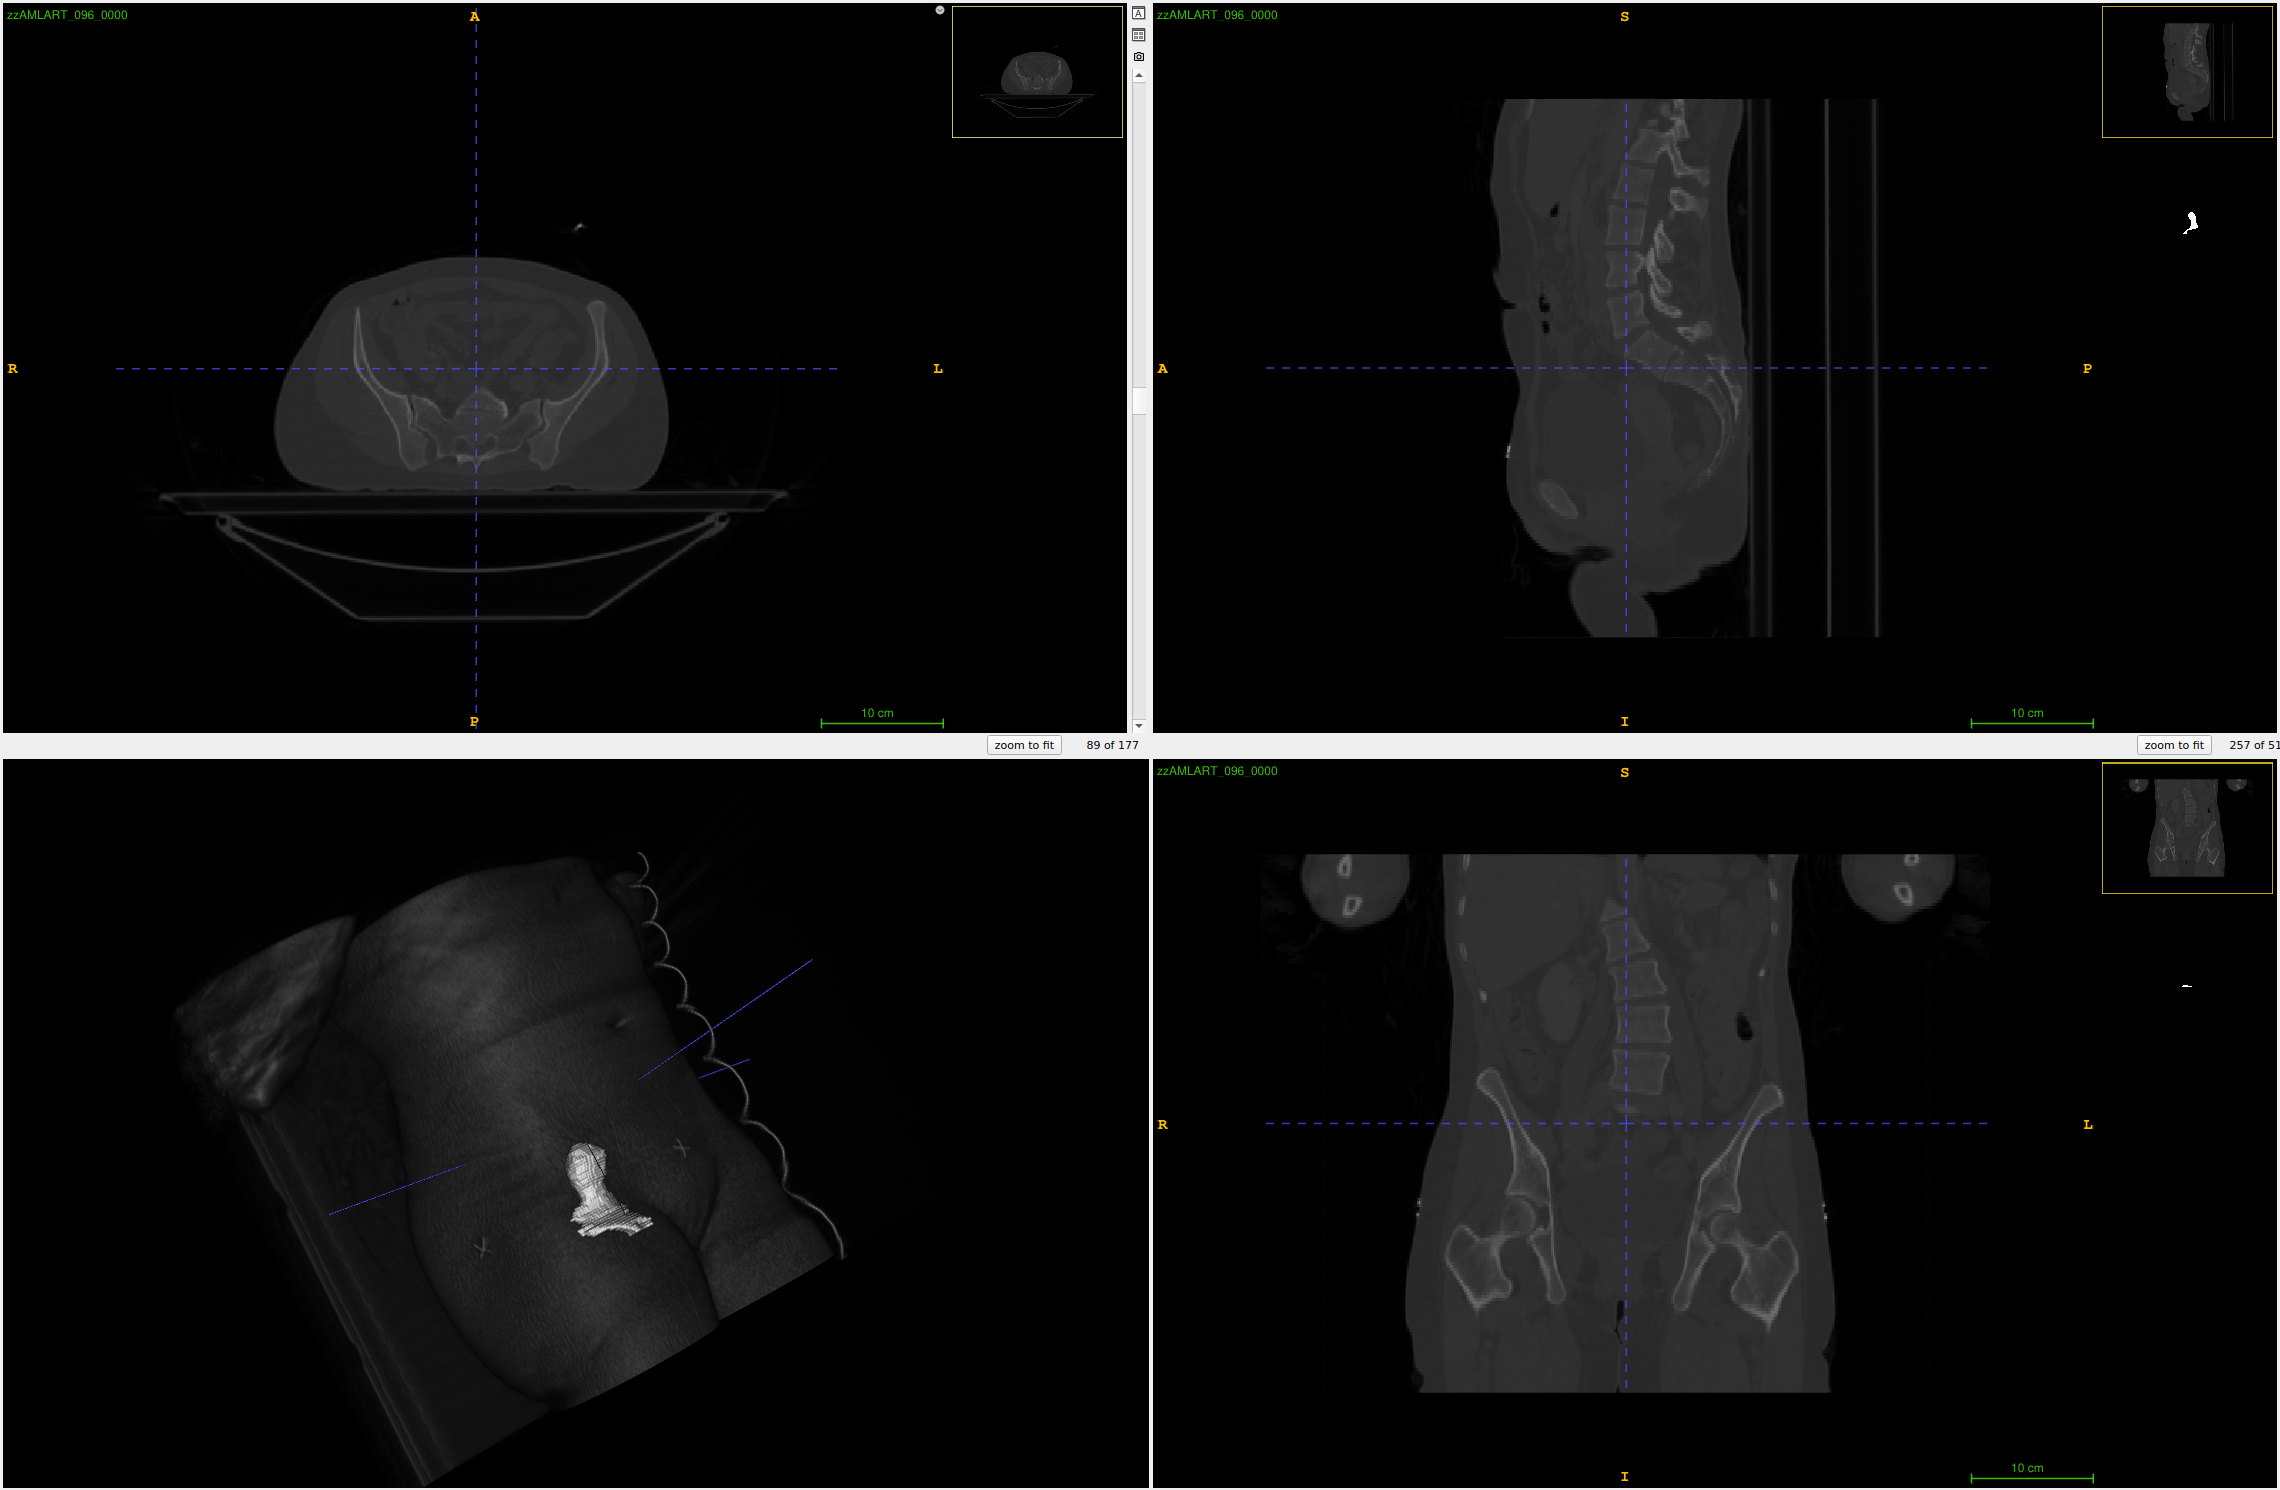
\includegraphics[width=0.7\linewidth]{../figures/CTVp.png}
  \captionof{figure}{The CTVp of an arbitrary patient}
  \label{fig:example-CTVp}
\end{figure}

\textbf{CTVp} stands for Primary Clinical Target Volume, see the example at Figure \ref{fig:example-CTVp}. This is the CTV where there may be local microscopic spread (uterus, cervix, upper vagina, primary tumour) \cite{AMLART-data}. This is the area that contains the tumour.

It is made from the following structures:

\begin{itemize}
    \item GTVp - Primary gross tumour volume (Visible Primary Tumour)
    \item Whole cervix (this will contain at least most of the GTVp. The GTVp could however grow out of this structure)
    \item Uterus - (contains the whole cervix)
    \item Vagina for CTV - (2cm below the lowest slice containing the cervix or GTVp). The whole vagina is initially contoured, then the vagina for CTV is made by copying the whole vagina and deleting unnecessary slices. 
\end{itemize}

We have that $Whole\ Cervix + GTVp = High\ Risk\ CTV$ which clinitians advise may be easier to train on since the GTVp will be harder to learn due to large variation in samples.

We also have that $High\ risk\ CTV + Uterus + vagina\ for\ CTV = CTVp$

\subsubsection{CTVn}\label{sec:data-CTVn}

\begin{warning}
  Find better figure for this
\end{warning}

\begin{figure}[H]
  \centering
  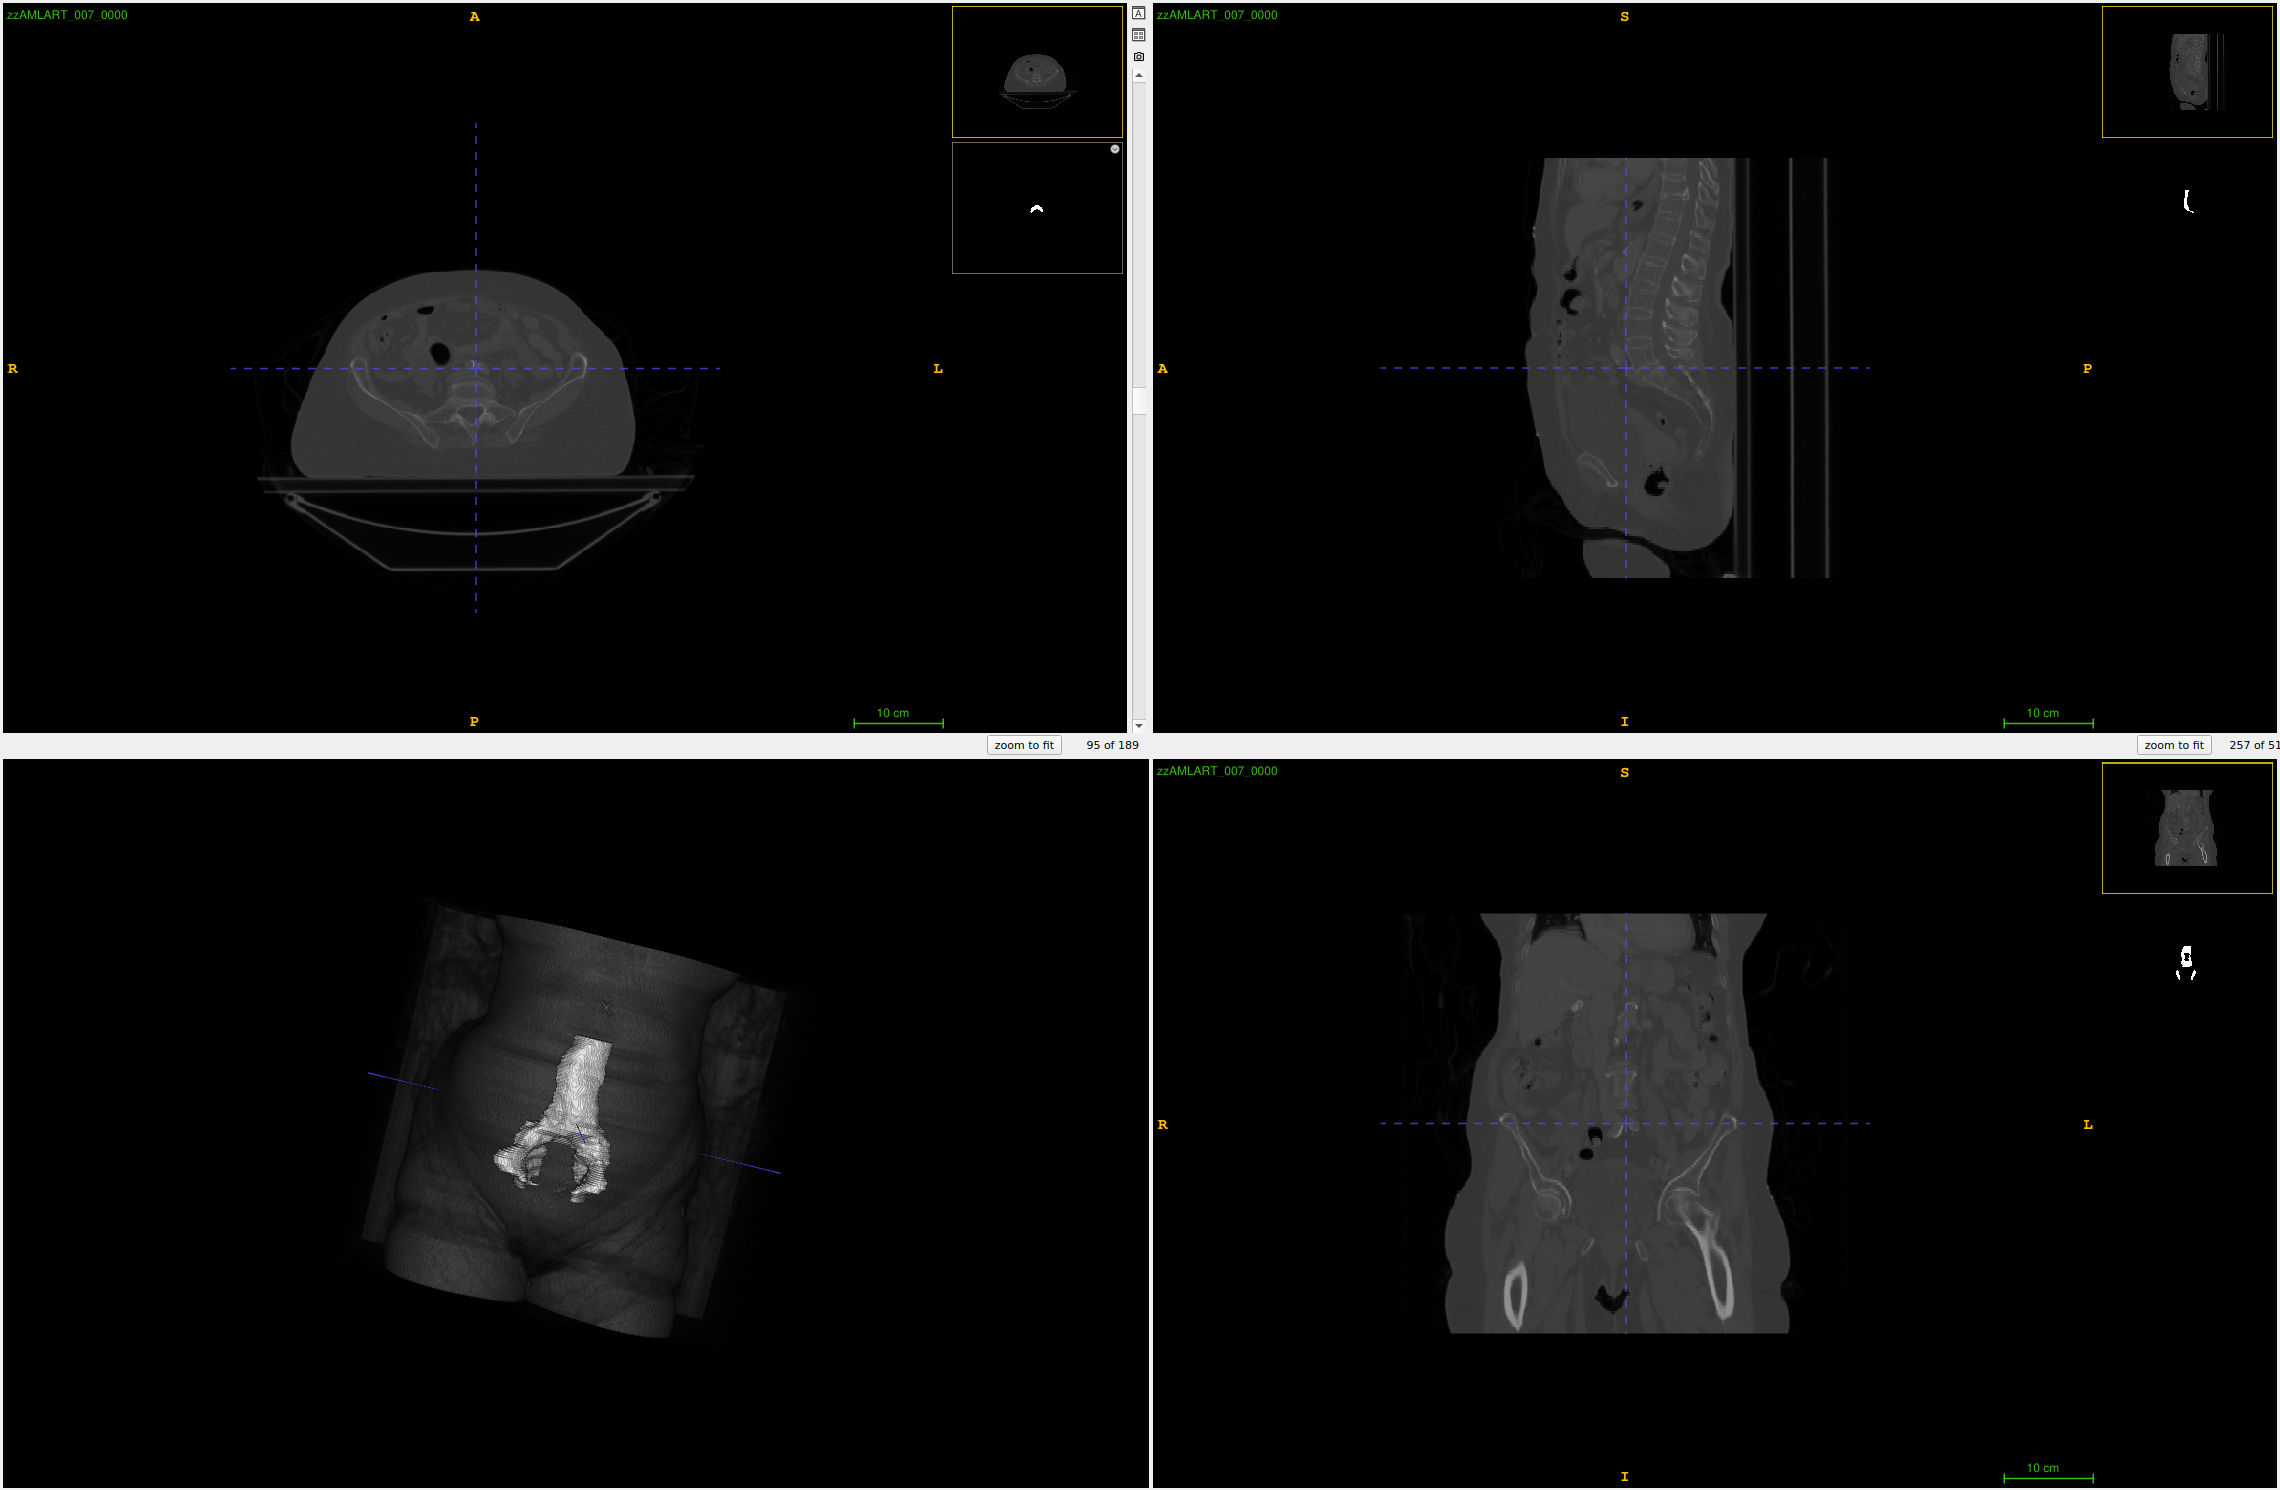
\includegraphics[width=0.7\linewidth]{../figures/CTVn.png}
  \captionof{figure}{The CTVn of an arbitrary patient}
  \label{fig:example-CTVn}
\end{figure}

\textbf{CTVn} stands for Nodal Clinical Target Volume see the example at Figure \ref{fig:example-CTVn}. This is the CTV where there may be microscopic spread to lymph nodes. It is drawn based on set margins around pelvic blood vessels and includes pelvic lymph nodes, common iliac lymph nodes and para-aortic lymph nodes \cite{AMLART-data}.

There are three groups of lymph nodes. In clinical practice, the number of these groups included in the CTV varies in each patient, depending on how advanced the disease is. Pathological lymph nodes (GTVn) are also included

\begin{itemize}
    \item Pelvic lymph nodes
    \item Common iliac lymph nodes
    \item Para-aortics
    \item GTVn (Gross Nodal Tumour) (usually included within the CTV nodes)
\end{itemize}

We have that $GTVn + Common\ iliac + pelvic + para-aortics = Nodal\ CTV$

\subsubsection{Parametrium}\label{sec:data-Parametrium}

\begin{warning}
  Find better figure for this
\end{warning}

\begin{figure}[H]
  \centering
  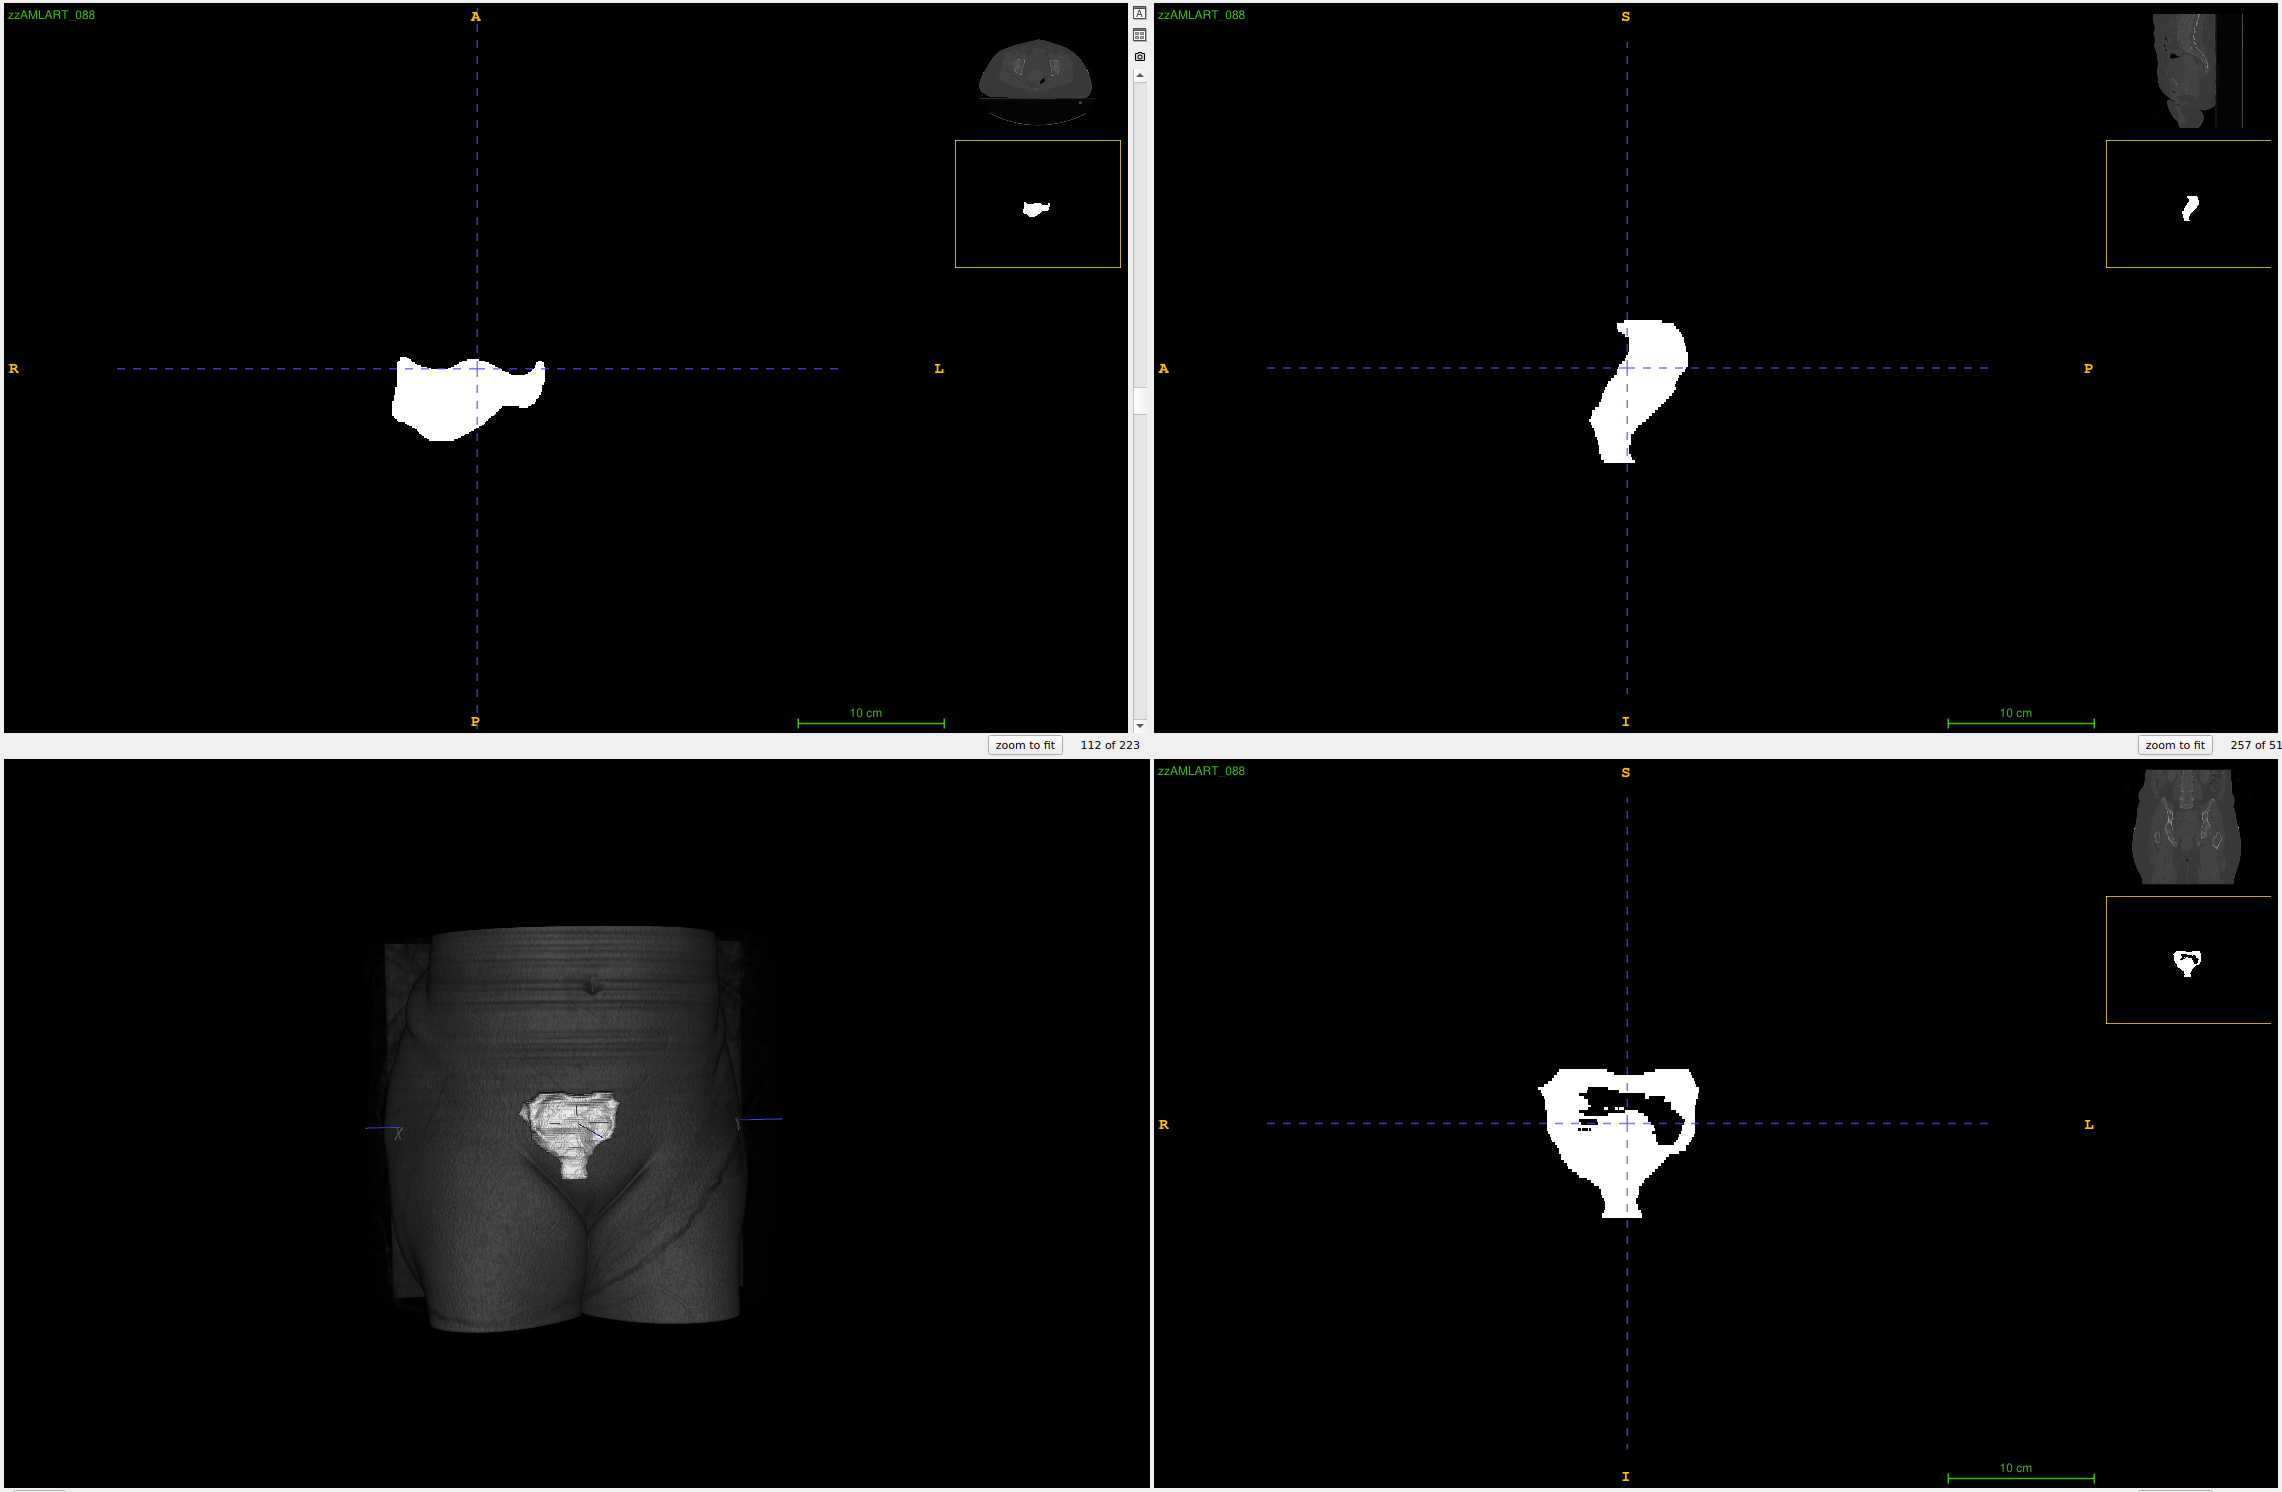
\includegraphics[width=0.7\linewidth]{../figures/Parametrium.png}
  \captionof{figure}{The Parametrium of an arbitrary patient}
  \label{fig:example-parametrium}
\end{figure}

\textbf{Parametrium/ Paravagina} is the tissue surrounding the cervix/vagina - at risk of local spread, see Figure \ref{fig:example-parametrium}. Drawn as a complete structure, then also to the level of the vagina included in the CTVp \cite{AMLART-data}.

Parametrium and Paravagina (whole and for CTV)  Contour whole Parametrium and Paravagina. Parametrium and Paravagina for CTV can be made by copying the whole paravagina and editing back to the level of vagina to be included.

\subsection{Data Cleaning}\label{sect:data-cleaning}

\section{Evaluation Metrics}\label{sect:evaluation-metrics}

\subsection{Geometric}\label{sect:geometric}

\subsection{Honorable mentions}\label{sect:evaluation-metrics-honorable-mentions}

\section{Baseline Results}\label{sect:baseline-results}

\begin{warning}
  TODO for all
\end{warning}

\subsection{nnU-Net}\label{sect:results-nnu-net}

\subsection{Total Segmentator}\label{sect:results-totalseg}

\subsection{UinverSeg}\label{sect:results-universeg}

\section{Summary}\label{sect:results-summary}

%%%%%%%%%%%%%%%%%%%%%%%%%%%%%%%%%%%%
\chapter{Proposal}\label{sect:proposal}

\begin{warning}
  Should we keep labels individual and segment them separately or should we segment it all in one shot?
\end{warning}

\begin{warning}
  Solution to resolution problem, down-sample all samples or think of average?
\end{warning}

%%%%%%%%%%%%%%%%%%%%%%%%%%%%%%%%%%%%
\chapter{Ethics}\label{sect:ethics}

This project involves very intimate and personal information of many female patients. Researchers may collaborate with third-parties by providing anonymized data which may not be reverse engineered back to the patient.
The lack of this effort may result in ``stigma, embarrassment, and discrimination'' \cite{health-privacy} if the data is misused.

\section{Patient disclosures}\label{sect:patient-disclosures}

The Royal Marsden Hospital doesn't require ``explicit consent'' for sharing collected clinical data with outside entities as long as the patient is made aware of the ways their ``de-identified/anonymized'' data may be used  \cite{royal-marsden-privacy-note}. Formalities are also arranged with Imperial Collage's Medical Imaging team such as acting as ``ethical data stewards'' \cite{ethics-imaging-AI}. Without such disclosure and anonymisation of data, patients may be reluctant to provide candid and complete disclosures of their sensitive information, even to physicians, which may prevent a full diagnosis if their data isn't maintained in an anonymous fashion.

The MIRA team acts as responsible data stewards by storing anonymized data within a folder on the college network. All provided data was anonymized by the Royal Marsden Hospital and sent to team MIRA in the \texttt{NIfTI} file format which discloses no personal identifiable information, as defined by GOV website \cite{gov-gdpr}. This folder contains security measures which limit the availability of data only to those with specific access rights. Furthermore, operating on the preamble of de-identified data further reduces individual patient risk in the event that data is ever brought outside the confines of this folder.

\section{Using the tool}

The applications of this tool bode well in the healthcare ecosystem as the community slowly realizes the importance of AI-powered tools for the next generation of medical technology. Radiology has been one application that has been most welcoming of the new advances in technology as there is potential for substantial aid by reducing manual labor, increasing precision and freeing up the primary care physician's time \cite{overview-of-ai-medicine}.

Yet, it is too early to take result the medical tool as gospel. For current cervical radiotherapy delineation tools, only 90\% of the output is considered as acceptable for clinical use \cite{auto-delineation-cervical-cancer-development}. The remainder therefore has the potential to cause more harm than good if not checked properly. For example, overlap of a PTV onto an organ-at-risk may invoke a cascade of negative effects for the patient. A potential cause may be the lack of multivariate analysis, where an oncologist would need to consider a variety of data, whereas this model only considers a single point of evidence (results of an imaging modality).

Therefore, a degree of supervision required from physicians has to be established if this tool is to be used in practice. Oncologists will be required to reverse-engineer results of the `black-box' to verify why a decision has been made. Secondly, the responsible party for incorrect decisions made by DL tools should also be determined \cite{AI-in-cancer-diagnosis-era}.

%%%%%%%%%%%%%%%%%%%%%%%%%%%%%%%%%%
\printbibliography
\addcontentsline{toc}{chapter}{Bibliography}

\end{document}